\documentclass[12pt, letterpaper]{article}
\usepackage[utf8]{inputenc}
\usepackage{caption}
\usepackage{subcaption}
\usepackage{graphicx}
\usepackage{listings}
\usepackage{xcolor}
\def\code#1{\texttt{#1}}
\graphicspath{{./Pictures/}}


\setlength{\parskip}{1em}

%Set up listing env

\usepackage{xparse}



\NewDocumentCommand{\codeword}{v}{\texttt{\textcolor{blue}{#1}}}

\lstset{language=C,keywordstyle={\bfseries \color{blue}}}

\lstset{language=C,keywordstyle={\bfseries \color{blue}}}


\title{Vacuum Meshing Guide}
\author{William Ellis}
\date{February 2022}

\begin{document}

\begin{titlepage}

\end{titlepage}
\section{How Does it Work?}
\subsection{Mesh Skinning}
The skinning algorithm is fairly straight forward. A loop is done over all the elements in the mesh, in which each face/edge of the element is checked to see if it has a neighbour. If the face/edge has no neighbor, then the local face ID is added to a list. This check is done for all the faces/edges. Once completed, the nodes belonging to all the faces/edges in the list are added to another list, and the connectivity data of these faces/edges stored in another list. The new skinned mesh is then constructed using the list of nodes and the stored connectivity data.
\begin{figure}
    \includegraphics[width=\linewidth]{}
	\caption{Example of skinning output using 2D mesh.}
	\label{2DSkinExample}
\end{figure}

\subsection{Vacuum Generation}
Vacuum generation is essentially a two step process; boundary generation, and tetrahedralisation. Boundary generation refers to the process of generating a boundary around the skinned mesh. Tetrahedralisation refers to the process of generating tetrahedra (or sometimes tri elements) in a well defined region. Boundary generation is necessary to well define the space in which tetrahedralisation will occur.

\subsubsection{Boundary Generation}
Boundary generation concerns generating a simple boundary around
\begin{figure}
    \includegraphics[width=\linewidth]{}
	\caption{Example of why the boundary mesh is necessary to generate the vacuum.}
	\label{Boundary Example}
\end{figure}


\subsubsection{Tetrahedralisation}

\subsection{Full Mesh Generation}
\section{Building}

\section{Using}
\subsection{Using the examples}
There are three examples built in to the repo. These examples utilise  the functionality found in the library to different extents, and should be enough for most users to do what they need.

\subsubsection{skinner}
The first example, the source of which can be found in problems/skinner.cpp, is an example of how to get the skin of a mesh. This example loads in an input mesh given by the user and utilises the function \codeword{getSurfaceMesh} to obtain the skin of the input mesh. This can be used with meshes composed of 2D or 3D elements. In the 2D case, the skinned mesh will be composed of 1D edge facets, representing the boundary of the 2D boundary. In the 3D case, the skinned mesh will be composed of 2D facets. 

\begin{figure}
	\begin{subfigure}{0.48\textwidth}
		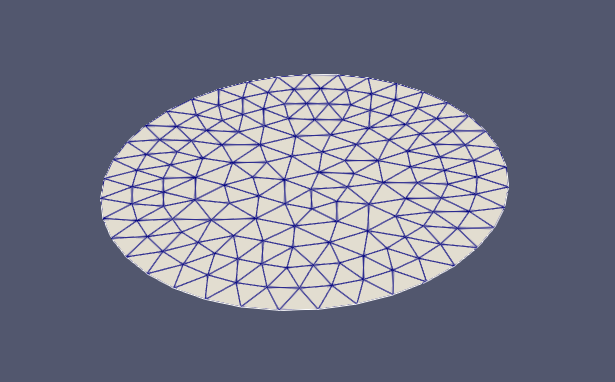
\includegraphics[width=\linewidth]{circleSurf.png}
		\caption{Before}
	\end{subfigure}
	\hspace*{\fill}	
	\begin{subfigure}{0.48\textwidth}
		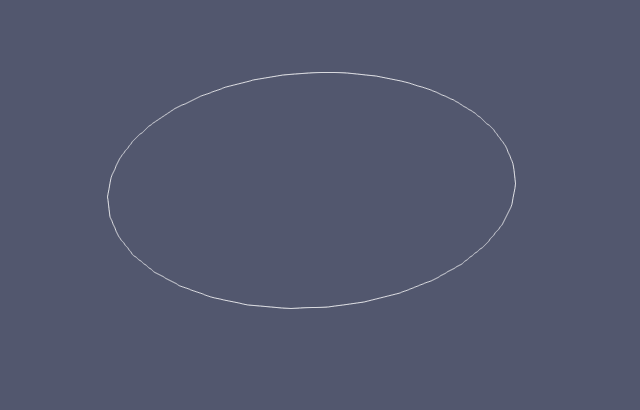
\includegraphics[width=\linewidth]{circleBound.png}
		\caption{After}
	\end{subfigure}	
	\caption{Example of skinning a mesh composed of 2D facets.}
	\label{2DSkinningComp}
\end{figure}

For example, if you had a mesh called `myMesh.e`, from the command line you could enter 
\begin{lstlisting}[language=bash]
	./build/examples/skinner -i Meshes/myMesh.e
\end{lstlisting}
to skin a mesh called myMesh. This should successfully save a mesh called MyMesh\verb|_|skin.e in the directory where the command was called from. 

\subsubsection{Generate Vacuum}
The second example included in the repo 

\subsection{Using the library}
As previously mentioned, the functionality found in this repo is built into a library called "VacuumMeshing". The example executables are linked to this library in order to utilise the funtionality. There is no reason that this library couldn't be linked to any of your own projects. Within the repo, naviating to "./VacuumMeshing/CMakeLists.txt" will show you how the library is built. The libIGL libraries that are linked in when the library is created have PUBLIC "inheretence". This means that any targets depending on this library will automatically be linked in with the necessary libIGL libs. This saves the user (you) having to mess around with ligIGL includes/libs. The MPI lib linked in with the library is set as PRIVATE, so that when building your own projects they will NOT link against the MPI version used to build the VacuumMeshing library.

\end{document}
